\section{Intermediate Memory Capacity Optimizes Spatial Navigation}

\subsection{Background}
Organisms navigating complex environments face a fundamental trade-off between exploration (gathering information) and exploitation (using knowledge to achieve goals efficiently) \cite{hills2015}. Spatial navigation research has traditionally focused on two strategies: \textbf{local heuristics} (simple rules based on immediate sensory input) and \textbf{cognitive maps} (mental representations enabling flexible path planning) \cite{tolman1948,okeefe1978}. Cognitive map formation requires extensive exploration to build complete spatial knowledge, after which animals should execute optimal paths with minimal further exploration.\\ \\
Rosenberg et al.\ (2021) demonstrated that water-deprived mice learned to navigate a binary tree maze after only $\approx 10$ reward experiences, yet continued spending 84\% of their time exploring rather than executing direct paths \cite{rosenberg2021}. This persistent exploration contradicts expectations for animals with complete cognitive maps, who should minimize exploration once spatial knowledge is acquired. Why do mice continue exploring so extensively if they can already navigate reliably?\\ \\
The authors observed that mice employed local navigation biases (alternation, branch preference, forward motion) and demonstrated accurate homing behavior. Critically, the binary tree structure permits successful homing through simple branch bias alone (Figure \ref{fig:branch})—a statistical preference for turning at junctions—which reliably guides animals back to the entrance without requiring explicit path memory.

\begin{figure}[h]
    \centering
    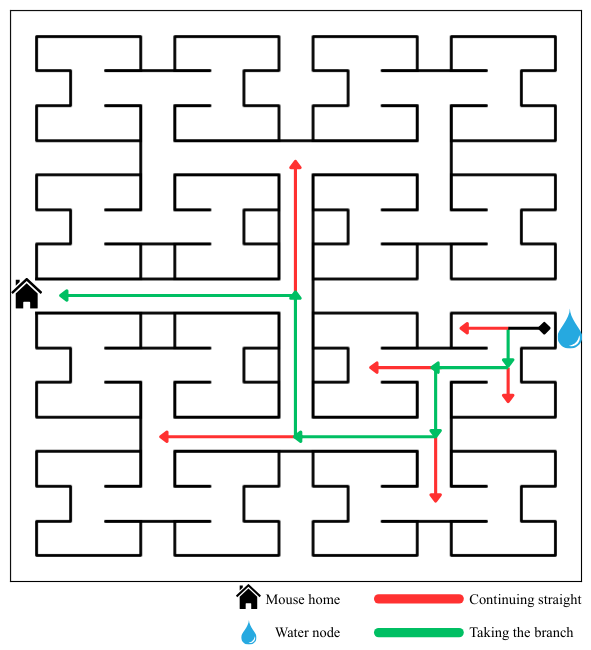
\includegraphics[width=0.5\textwidth]{figures/branch_bias.png}
    \caption{Example of a Navigation heuristic: \textit{The Branch Bias} ensures reliable homing from any node in the binary tree maze through a statistical preference for turning at junctions. This simple heuristic requires no spatial memory yet enables one-shot homing.}
    \label{fig:branch}
\end{figure}

This suggests successful task completion does not require full cognitive map construction—mice may navigate effectively with far less spatial memory than traditionally assumed. If minimal memory suffices for homing and goal-finding, the 84\% exploration may reflect not a choice to explore despite having complete knowledge, but rather \textit{necessary} exploration due to incomplete spatial memory. Under this hypothesis, mice operate with intermediate memory capacity: sufficient for systematic search and reliable homing, but insufficient for planning optimal routes.

This extension addresses: \textit{how much memory capacity is required for efficient navigation, and which memory level produces exploration patterns consistent with the observed 84\%?} We implemented agents with varying spatial memory capacities—from purely reactive navigation (no spatial memory) through minimal memory buffers to complete cognitive maps—and measured both navigation performance and exploration. By varying the memory capacity while holding navigation strategies constant, we determine whether memory constraints alone can account for the persistent exploration observed in biological navigation.

\subsection{Methods}

\subsubsection{Environment}
We used a binary tree labyrinth (k=2, depth=6) matching Rosenberg et al. (2021): 63 T-junctions, 64 endpoints, one containing water reward. State space doubled (254 states) to represent search and return phases.

\subsubsection{Memory Hierarchy}

We tested six memory levels:\\
\textbf{Level 0 (Reactive, 224 bits):} No spatial memory. Navigation via local heuristics only: forward bias ($P_{SF} \approx 0.88$), alternation ($P_{SA} \approx 0.72$), branch bias ($P_{BS} \approx 0.54$). Includes dead-end avoidance and deterministic homing (always reverse when carrying water).\\
\textbf{Level 1a-1d (Ranging Memory, 864-4,288 bits):} Remembers visited nodes with varying buffer sizes:
\begin{itemize}
    \item L1a: 20 nodes (864 bits)
    \item L1b: 50 nodes (1,824 bits)
    \item L1c: 100 nodes (3,424 bits)
    \item L1d: Unlimited (4,288 bits)
\end{itemize}
These agents use the same heuristics as Level 0 but penalizes actions leading to frequently-visited nodes: $\text{penalty} = 0.5 \times \log(\text{visits} + 1)$. When the buffer is full, the oldest memories forgotten (via FIFO).\\
\textbf{Level 2 (Full Memory, 24,384 bits):} A tabular Q-learning Agent \cite{watkins1992} with complete state-action memory. This agent was trained until it reached 5 consecutive optimal episodes (12 steps). It represents a complete cognitive map.\\ \\
All agents evaluated over 50 trials with 10,000-step limit and loop detection (stuck if oscillating between $\leq 3$ states over 20 steps).

\subsection{Results}

\subsubsection{Memory Capacity and Performance}

Table \ref{tab:results} shows navigation performance across memory levels. Exploration rates vary with memory capacity. Interestingly, as memory capacity increases from L1a through L1d, exploration fraction decreases monotonically (76\% → 66\%), while paradoxically, task completion also degrades (90\% → 46\%). Rosenberg et al.\ observed 84\% exploration time in mice. None of our memory-limited agents approach the 84\% exploration observed in mice, though the closest matches occur at minimal memory capacities that reached the 74-76\% mark. Level 2 agents with complete cognitive maps exhibit minimal exploration (6\%) after training, consistent with map-based navigation suppressing exploration once spatial knowledge is acquired. These results suggest that the 84\% exploration may reflect memory constraints beyond those tested here, or alternatively, may arise from mechanisms other than simple capacity limitations.

\begin{table}[h]
\centering
\begin{tabular}{lccccc}
\toprule
Level & Type & Memory (bits) & Completion & Exploration & Steps \\
\midrule
L0 & Reactive & 224 & 36\% & 40\% & 3,405 \\
L1a & 20 nodes & 864 & 90\% & 76\% & 1,736 \\
L1b & 50 nodes & 1,824 & 72\% & 74\% & 2,170 \\
L1c & 100 nodes & 3,424 & 62\% & 69\% & 2,098 \\
L1d & Unlimited & 4,288 & 46\% & 66\% & 2,160 \\
L2 & Full Memory & 24,384 & 100\% & 6\% & 12 \\
\bottomrule
\end{tabular}
\caption{Navigation performance across memory levels (50 trials each).}
\label{tab:results}
\end{table}

\subsubsection{Intermediate Memory Outperforms Unlimited}

Figure \ref{fig:2panel} shows a U-shaped relationship between memory capacity and navigation efficiency. 

\begin{figure}[h]
    \centering
    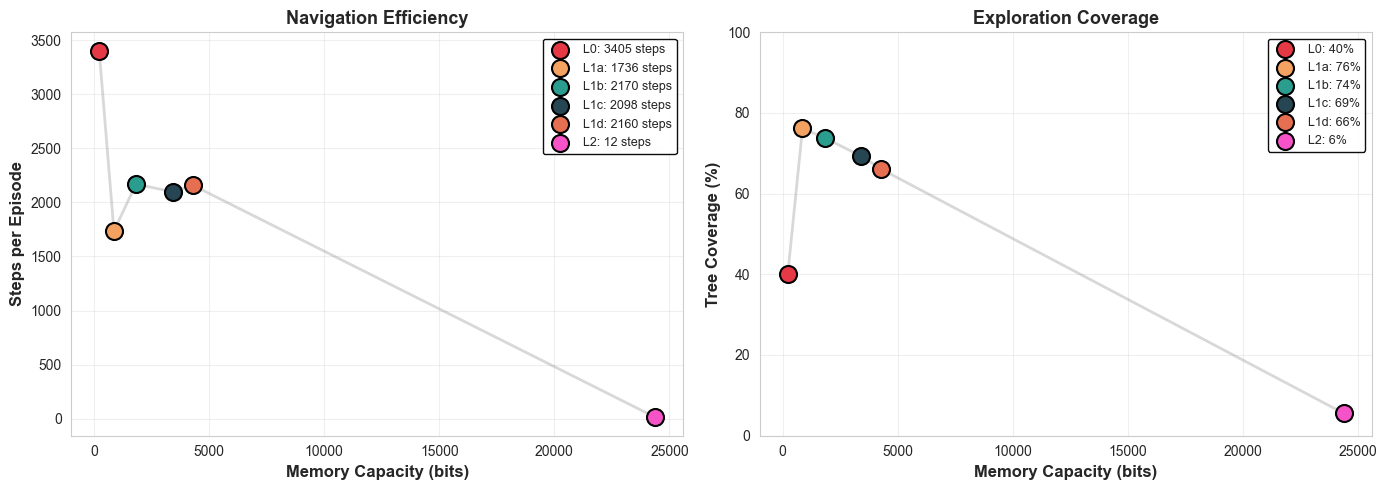
\includegraphics[width=\textwidth]{figures/2panel.png}
    \caption{\textbf{Left:} Steps per episode vs.\ memory capacity shows optimal performance at intermediate memory (L1b, 1,824 bits). Greater memory (L1c, L1d) leads to \textit{worse} performance. \textbf{Right:} Tree coverage remains high across all memory levels, indicating the performance difference reflects navigation strategy, not exploration failure.}
    \label{fig:2panel}
\end{figure}

\textbf{Key findings:}
\begin{itemize}
    \item \textbf{Memory enables navigation:} L0 (no memory) achieves only 36\% completion. Adding minimal memory (L1a, 20 node memory capacity) raises completion to 90\%.
    
    \item \textbf{Intermediate memory is optimal:} L1a (20 node memory capacity, 864 bits) completes 90\% of trials in 1,736 steps—20\% faster than unlimited memory (L1d: 2,160 steps), despite using only 20\% of L1d's memory capacity.
    
    \item \textbf{More memory degrades performance:} Beyond 50 nodes, increasing memory capacity leads to longer, less efficient paths. L1c (100 node memory capacity) requires 2,098 steps and achieves only 62\% completion.
\end{itemize}

\subsubsection{Task Completion Across Memory Levels}

Figure \ref{fig:completion} shows completion rates improve dramatically with minimal memory (L0: 36\% → L1a: 90\%) but then or decline with additional capacity.

\begin{figure}[h]
    \centering
    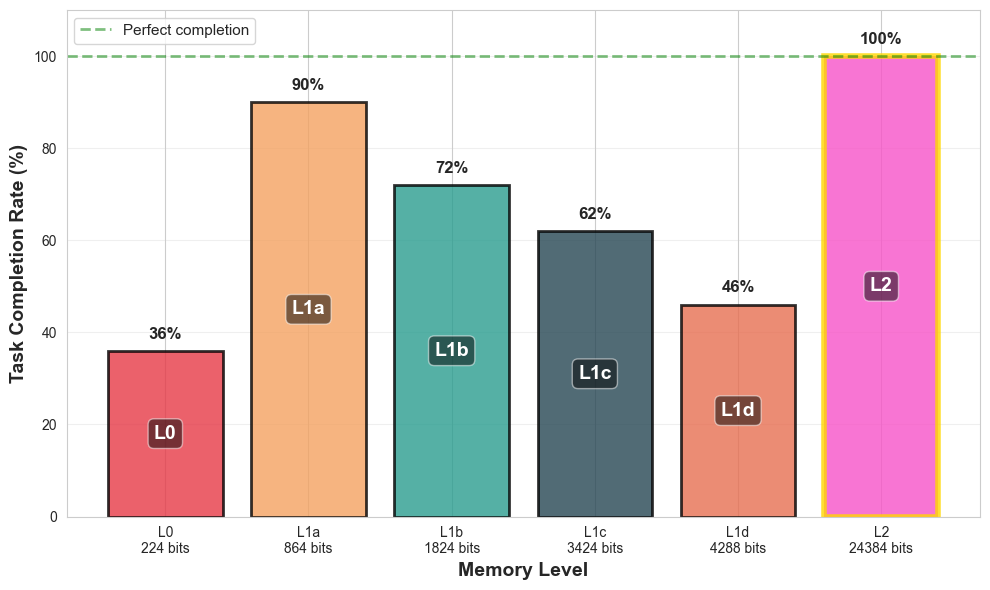
\includegraphics[width=0.8\textwidth]{figures/bar_graph1.png}
    \caption{Task completion rates across memory levels. Minimal memory (L1a) achieves satisfactory performance; excessive memory (L1c-L1d) shows degradation.}
    \label{fig:completion}
\end{figure}

\section{Discussion}

\subsubsection{Why Minimal Memory Outperforms Larger Buffers}

Our results reveal a counterintuitive pattern: the smallest memory buffer tested (L1a, 20 nodes) achieves superior performance to all larger capacities. With unlimited memory (L1d, 4,288 bits), visit counts accumulate indefinitely. The novelty penalty ($0.5 \times \log(\text{visits})$) increasingly suppresses actions toward familiar areas. After visiting a node 10+ times, agents actively avoid it, even when navigation requires passing through familiar territory. This creates inefficient, circuitous routes and reduces completion rate to 46\%. \\ \\
With minimal memory (L1a, 20 nodes), only the most recent visits are retained via FIFO (First in - First out) replacement. Agents maintain flexibility to backtrack and navigate through previously-explored space without excessive penalties. This achieves 90\% task completion in 1,736 steps—20\% faster than unlimited memory despite using only one-fifth the capacity (864 vs.\ 4,288 bits).\\ \\
Intermediate buffers (L1b-L1c) show mediocre performance, suggesting that very small memory is sufficient for this task structure, while larger buffers introduce detrimental over-penalization of familiar paths without providing commensurate benefits.

\subsubsection{Biological Implications}

Our results suggest \textbf{minimal spatial memory may be sufficient for efficient navigation in structured environments}. Forgetting serves critical functions \cite{anderson2021,norby2015,ryan2022}:

\begin{itemize}
    \item \textbf{Maintains flexibility:} Prevents over-avoidance of familiar but necessary paths \cite{pravosudov2018}
    \item \textbf{Enables systematic exploration:} L1a achieves 76\% exploration while maintaining 90\% completion
    \item \textbf{Optimizes resource allocation:} L1a achieves superior performance with minimal memory investment (864 bits vs.\ 4,288 bits for unlimited)
\end{itemize}

\subsubsection{Comparison with the 84\% Exploration}

Rosenberg et al.\ observed 84\% exploration time in mice. Our framework reveals:
\begin{itemize}
    \item \textbf{Level 0} (no memory): 40\% exploration, but only 36\% task completion, insufficient for reliable navigation.
    \item \textbf{Level 1a} (20 nodes): 76\% exploration with 90\% completion, closest to biological behavior.
    \item \textbf{Level 1b-1d} (50-unlimited nodes): 74-66\% exploration, decreasing with memory capacity
    \item \textbf{Level 2} (full map): 6\% exploration after training, map based navigation suppresses exploration
\end{itemize}

Notably, none of our memory-limited agents reach the 84\% exploration observed in mice. The closest match (L1a: 76\%) still falls 8 percentage points short, suggesting that mice either operate under even tighter memory constraints than 20 nodes, employ qualitatively different exploration strategies, or face environmental uncertainties not captured in our deterministic maze structure. The systematic decrease in exploration fraction as memory capacity increases (76\% → 66\%) confirms that memory constraints promote exploratory behavior.

\subsubsection{Limitations}

Our novelty penalty weight (0.5) was selected empirically; biological systems may dynamically modulate exploration based on task demands or uncertainty. Additionally, we assume perfect memory fidelity within capacity limits; neural noise and synaptic interference may effectively reduce functional buffer sizes below nominal capacity \cite{kitamura2018,akers2014}. The deterministic maze structure lacks environmental uncertainty that might sustain exploration in biological contexts. Finally, our agents employ FIFO replacement; biological forgetting may follow different dynamics (recency-weighted, context-dependent, or interference-based) \cite{ryan2022}.
